\title{Matrix Multiplication}
\date{}

\documentclass[12pt]{article}

\usepackage[italian]{babel}
\usepackage[T1]{fontenc}
\usepackage[utf8]{inputenc}
\usepackage{graphicx}
\usepackage{amsmath}
\usepackage{amssymb}
\usepackage{float}

\begin{document}
\maketitle
\newpage

\section{Introduzione}
L'\emph{assignment} prevede il calcolo del prodotto matriciale tra due matrici di dimensione $N \times N$ mediante varie strategie:
\begin{itemize}
\item CPU
\item GPU tramite \emph{global memory}
\item GPU tramite \emph{shared memory}
\item Più GPU
\end{itemize}

La \emph{shared memory} si stima essere circa $100$ volte più veloce della \emph{global memory} per cui è lecito aspettarsi un notevole miglioramento utilizzando tale tecnica. Si è scelto di sfruttare la \emph{shared memory} anche nell'implementazione che sfrutta più GPU.

\subsection{Moltiplicazione a blocchi}
Per le due implementazione che sfruttano la \emph{shared memory} si è utilizzata la moltiplicazione matriciale a blocchi. La matrice viene divisa in blocchi di dimensione$ 32 \times 32 $ in modo che ogni blocco possa essere memorizzato nella memoria condivisa da un blocco di thread della stessa dimensione e computato separatamente.  La GPU \emph{Tesla K40c} utilizzata per le prove mette a disposizione $49152 byte$ per blocco, assicurando la possibilità di sfruttare blocchi della dimensione scelta, in quanto:
$$ (32)^2 \cdot sizeof(int) = 32768 byte < 49152 byte $$
Anche la scheda video \emph{GeForce GTX 750} che viene impiegata nella versione con due GPU ha la stessa dimensione di memoria condivisa per blocco, per cui non è stato necessario rivalutare la strategia.

\section{Parallelizzazione}
La moltiplicazione è di per sé un'operazione che permette di calcolare ogni singolo elemento della matrice in modo indipendente dagli altri, almeno utilizzando l'algoritmo più semplice. Per cui nella versione che usa la GPU per rendere il calcolo parallelo usando la memoria globale è stato sufficiente inizializzare $N \times N$ blocchi da 1 thread ciascuno per eseguire il calcolo.

Le due versioni con memoria condivisa hanno invece necessitato la creazione di $N/32 \times N/32$ blocchi con $32 \times 32 $ thread ciascuno. Ogni blocco esegue il compito di calcolare gli elementi appartenenti allo stesso blocco della matrice risultante.

Infine, per quanto riguarda la versione con due GPU si è divisa in due la matrice del \emph{moltiplicatore} e del \emph{prodotto}, in tal modo è stato sufficiente passare una singola metà di entrambe le matrici a ciascuna GPU. La matrice del \emph{moltiplicando} è stata invece passata ad entrambe le GPU, poiché per computare mezzo prodotto è necessario conoscerla completamente.

\section{Benchmark}
Si presenta ora il grafico relativo a tutti i test eseguiti sulle varie implementazioni dell'algoritmo, al crescere di $N$:
\begin{figure}[h]
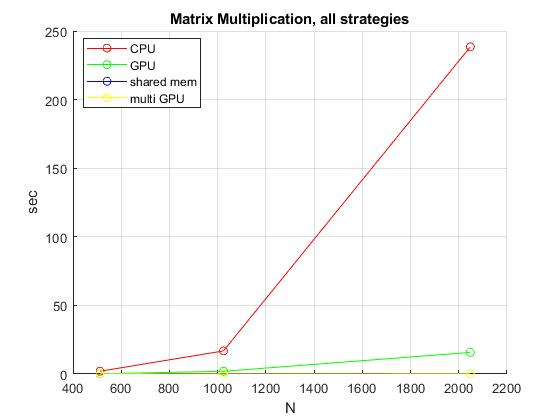
\includegraphics[width=\textwidth]{MatrixMul_all.jpg}
\centering
\end{figure}

Si nota come la versione che sfrutta la CPU risulti nettamente meno performante delle versioni che sfruttano la GPU. Un ulteriore salto di qualità è visibile con l'ausilio della \emph{shared memory}.

Al fine di evidenziare le differenza tra l'implementazione con una e due GPU si può visionare il seguente grafico che le compara separatamente:
\begin{figure}[h]
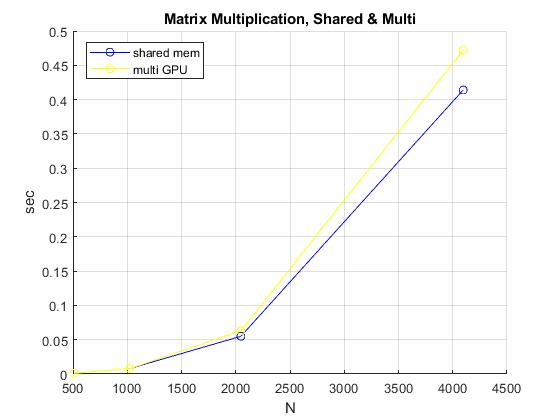
\includegraphics[width=\textwidth]{MatrixMul_sm.jpg}
\centering
\end{figure}

La versione con singola GPU risulta essere leggermente più performante della versione con due GPU, questo è giustificato dal fatto che la \emph{GeForce GTX 750} abbia prestazioni leggermente inferiori e il programma deve attendere che entrambe le schede video abbiano terminato la computazione prima di terminare.

\section{Conclusioni}
\'E stato possibile notare come la \emph{shared memory} impatti sensibilmente sulle performance è some l'utilizzo di due GPU non è necessariamente vantaggioso. Con due GPU si possono ottenere, tuttavia, vantaggi nel caso in cui la matrice fosse di dimensione molto elevata tale da dover richiedere più cicli di computazioni causa il limitato numero di blocchi della GPU.


\end{document}
